%% English report -- Elsevier CAS single-column (cas-sc)
\documentclass[a4paper,fleqn]{cas-sc}

\usepackage[numbers,sort&compress]{natbib}
\usepackage{amsmath,amssymb}
\usepackage{booktabs}
\usepackage{graphicx}
\usepackage{multirow}
\usepackage{xcolor}

\graphicspath{{../figures/}}

\shorttitle{Exact SAT Encoding for N-Queens}
\shortauthors{T.D. Duc}

\begin{document}
\let\WriteBookmarks\relax
\def\floatpagepagefraction{1}
\def\textpagefraction{.001}

\title[mode=title]{Exact SAT Encoding for the N-Queens Problem:\newline
An Empirical Comparison with MIP and CP}

\author[1]{Truong Dinh Duc}

\affiliation[1]{organization={Faculty of Information Technology,
  VNU University of Engineering and Technology},
  city={Hanoi}, postcode={100000}, country={Vietnam}}

\begin{abstract}
The N-Queens problem asks for a placement of $n$ non-attacking queens on an
$n\times n$ board and is a classical testbed for combinatorial solving. We
present an exact SAT-based approach that encodes N-Queens through
at-most-one (AMO) and at-least-one (ALO) cardinality constraints, and we study
how the choice of cardinality encoding interacts with the choice of SAT solver.
We implement five encodings from scratch (pairwise, binary, commander, product,
sequential) and seven encodings available in PySAT, and we evaluate eight SAT
solvers on instances with $n=8$ up to $n=80$ (three repetitions, 600\,s time
limit). We compare the SAT approach against seven exact baselines implemented
with Gurobi, CPLEX (MIP and CP), OR-Tools CP-SAT, OR-Tools MIP (SCIP), and
PuLP/CBC. The experiments show a strong encoding--solver interaction: the
pairwise encoding is the most robust and is dominant for weaker solvers, whereas
the binary encoding is fastest for strong solvers. MiniSat and MiniCard are the
most effective SAT solvers overall, while Glucose times out on the harder
encodings. Among the exact baselines, Gurobi is by far the fastest, with an
almost flat runtime, and CPLEX MIP is second; the best SAT configuration is
competitive with CP-SAT and CPLEX CP but clearly slower than the two commercial
MIP solvers on this feasibility-oriented problem.
\end{abstract}

\begin{keywords}
N-Queens \sep SAT encoding \sep cardinality constraints \sep AMO \sep PySAT \sep
MIP \sep constraint programming \sep empirical evaluation
\end{keywords}

\maketitle

\section{Introduction}\label{sec:intro}
The N-Queens problem consists in placing $n$ queens on an $n\times n$ chessboard
so that no two queens attack each other, i.e., no two queens share a row, a
column, or a diagonal. It is a well-known constraint satisfaction problem that
has been studied for decades both for its combinatorial structure and as a
benchmark for exact and heuristic algorithms \citep{BellStevens2009}. Although
the existence of a solution is known for every $n \geq 4$, finding a
satisfying placement and comparing the efficiency of different exact technologies
remain useful case studies.

Modern Satisfiability (SAT) solvers, based on conflict-driven clause learning
(CDCL) \citep{MarquesSilva1999}, have become an effective engine for a wide range
of combinatorial problems. N-Queens can be encoded into conjunctive normal form
(CNF) by representing each board cell by a Boolean variable and by expressing the
attacking constraints and the ``one queen per row'' condition as cardinality
constraints. The efficiency of the resulting CNF depends heavily on the encoding
of the at-most-one (AMO) and at-least-one (ALO) constraints
\citep{Sinz2005,Prestwich2009,KlieberKwon2007}.

In this work we ask how the choice of cardinality encoding interacts with the
choice of SAT solver, and how SAT compares with other exact paradigms such as
Mixed-Integer Programming (MIP) and Constraint Programming (CP) on N-Queens.
Our contributions are as follows.
\begin{itemize}
  \item We implement five AMO encodings from scratch (pairwise, binary,
        commander, product, and the sequential-counter encoding of Sinz) and use
        seven encodings provided by the PySAT library, within a single reusable
        Python package.
  \item We benchmark eight SAT solvers (MiniSat, MiniCard, CaDiCaL 1.5.3 and
        1.9.5, MergeSAT, Lingeling, Glucose 3 and 4) on instances from $n=8$ to
        $n=80$ with three repetitions and a 600\,s time limit.
  \item We compare SAT with seven exact baselines built with Gurobi, CPLEX (MIP
        and CP), OR-Tools CP-SAT, OR-Tools MIP (SCIP backend), and PuLP (CBC
        backend).
  \item We report and discuss a strong encoding--solver interaction, a
        solver-specific preprocessing artefact, and the gap between SAT and
        commercial MIP/CP solvers on this problem.
\end{itemize}

The rest of the paper is organized as follows. Section~\ref{sec:background}
defines the problem, reviews cardinality encodings, and discusses related work.
Section~\ref{sec:method} presents the CNF model, the encodings, the solver
harness, and the baselines. Section~\ref{sec:experiments} reports the
computational experiments and discusses the results. Section~\ref{sec:conclusion}
concludes.

\section{Background}\label{sec:background}

\subsection{Problem definition and CNF model}
Let $x_{r,c}$ be a Boolean variable that is true if and only if a queen is placed
in row $r$ and column $c$, for $0 \leq r,c < n$, so that $n^2$ variables are
used. A valid placement satisfies the following constraints:
\begin{align}
  \sum_{c=0}^{n-1} x_{r,c} &= 1 && \forall r \quad \text{(exactly one per row)},\\
  \sum_{r=0}^{n-1} x_{r,c} &\leq 1 && \forall c \quad \text{(at most one per column)},\\
  \sum_{\substack{(r,c)\in D}} x_{r,c} &\leq 1 && \forall \text{diagonal } D ,
\end{align}
where a diagonal is a maximal set of cells with constant $r-c$ (main diagonals)
or constant $r+c$ (anti-diagonals). Because every row contains exactly one queen,
there are exactly $n$ queens; consequently the column and diagonal constraints
only need the ``at most one'' direction. The exactly-one condition of a row is
encoded as the conjunction of an ALO constraint and an AMO constraint, while
columns and diagonals require only an AMO constraint.

\subsection{Cardinality encodings}
An AMO constraint over literals $\ell_1,\dots,\ell_m$ states that at most one
literal is true, and an ALO constraint states that at least one literal is true.
We consider the following AMO encodings, where $m$ is the number of literals.
\begin{itemize}
  \item \textbf{Pairwise.} One clause $(\neg \ell_i \vee \neg \ell_j)$ for every
        unordered pair $\{i,j\}$: $\binom{m}{2}$ clauses, no auxiliary
        variables. Propagation is strong but the CNF is large.
  \item \textbf{Binary.} Each literal is assigned a distinct $\lceil \log_2 m
        \rceil$-bit code and implications force the code; this uses
        $m\lceil\log_2 m\rceil$ clauses and $\lceil\log_2 m\rceil$ auxiliary
        variables.
  \item \textbf{Commander.} Literals are partitioned into groups of size at most
        $g$; each group gets a commander variable, AMO is enforced inside each
        group and among the commanders, recursively. This reduces the clause
        count to $O(m)$ at the cost of additional variables.
  \item \textbf{Product.} Literals are arranged on a $p\times q$ grid ($pq \geq
        m$); implications relate each literal to a row and a column variable, and
        AMO is enforced on the row and column variables.
  \item \textbf{Sequential (Sinz).} A chain of $m-1$ auxiliary variables encodes
        ``the number of true literals seen so far is at most one'', using
        $3m-4$ clauses and $m-1$ auxiliary variables; this is the standard
        sequential-counter encoding \citep{Sinz2005}.
\end{itemize}
In addition, PySAT \citep{Ignatiev2018} provides the \emph{bitwise},
\emph{ladder}, \emph{sorting-network}, \emph{cardinality-network}, and
\emph{totalizer} encodings, which we include for completeness. The clause and
variable counts of each encoding for $n=40$ are reported in
Table~\ref{tab:structure}.

\subsection{Related work}
N-Queens has a long history in combinatorics \citep{BellStevens2009}, and its
decision version (N-Queens Completion) has been shown to be NP-complete
\citep{Gent2017}, which motivates generic exact solvers. On the SAT side,
cardinality encodings are a central topic in the Handbook of Satisfiability
\citep{Biere2021,Prestwich2009}, with the sequential counter of Sinz
\citep{Sinz2005}, the pairwise and commander constructions
\citep{KlieberKwon2007}, and the binary and product variants
\citep{FrischGiannaros2010} being the most widely used. PySAT
\citep{Ignatiev2018} exposes these encodings through a uniform interface, and
modern CDCL solvers such as MiniSat \citep{EenSorensson2003}, Glucose
\citep{AudemardSimon2009}, and CaDiCaL/Kissat \citep{Biere2020} provide strong
search engines. On the optimization side, MIP and CP solvers such as Gurobi
\citep{Gurobi2024}, CPLEX \citep{IBM2022}, OR-Tools \citep{ORtools2023}, and CBC
\citep{ForrestCBC} are the standard exact baselines. Our study combines these
strands by systematically comparing cardinality encodings, SAT solvers, and
MIP/CP baselines on a single N-Queens model.

\section{Method}\label{sec:method}

\subsection{Model construction}
We build the CNF with rows encoded as exactly-one (ALO + AMO) and columns and
diagonals encoded as AMO, as described in Section~\ref{sec:background}. The
original variables occupy the identifiers $1,\dots,n^2$ and auxiliary variables
are allocated afterwards. Two diagonal encodings are provided: a \emph{naive}
mode that adds the pairwise clause $(\neg x_{r_1,c_1} \vee \neg x_{r_2,c_2})$ for
every pair of cells on a common diagonal (a quadratic expansion per diagonal),
and an \emph{optimal} mode that applies the selected AMO encoding once per
diagonal, which keeps the number of diagonals linear and reuses the same encoder.

\subsection{Encodings and solvers}
All five hand-written encodings and the seven PySAT encodings share one
interface, so that the same model can be instantiated with any encoding. Solving
is performed through PySAT; each solve is executed in an isolated subprocess so
that a crashing or hanging solver is recorded as \texttt{crash} or
\texttt{timeout} rather than aborting the experiment. For every run we record the
CNF build time, the solver time, the number of variables and clauses, and the
solver statistics (decisions, propagations, and conflicts).

\subsection{MIP/CP baselines}
The same N-Queens model is expressed with binary variables $a_{r,c}$ subject to
exactly-one per row, at-most-one per column, and at-most-one per diagonal, using
the following engines: Gurobi \citep{Gurobi2024}, CPLEX MIP and CPLEX CP
\citep{IBM2022}, OR-Tools CP-SAT \citep{ORtools2023}, OR-Tools MIP with the SCIP
backend, and PuLP with the CBC backend \citep{ForrestCBC}. All baselines minimise
a constant objective (the problem is a feasibility problem) and are run under the
same time limit as the SAT solvers.

\section{Computational experiments}\label{sec:experiments}

\subsection{Experimental setup}
All experiments were run on a Windows machine with an 11th-generation Intel
processor, using Python 3.11 and PySAT 1.8/1.9. We used the SAT solvers MiniSat
(\texttt{minisat22}), MiniCard (\texttt{minicard}), CaDiCaL 1.5.3 and 1.9.5,
MergeSAT 3, Lingeling, and Glucose 3 and 4. Instances range from $n=8$ to $n=80$
in steps of two. Each configuration was repeated three times and the median is
reported; the time limit is 600\,s per run. Two PySAT solvers available on some
platforms (\texttt{cryptosat}, \texttt{minisatgh}) were not shipped in the
distribution used here, and \texttt{kissat404} reproducibly crashes on these
instances; these solvers are therefore excluded. All reported instances are
satisfiable, so we measure the time to \emph{find} a model rather than to prove
unsatisfiability.

\subsection{CNF structure}
Table~\ref{tab:structure} shows the CNF size of each encoding for $n=40$. The
pairwise encoding uses the fewest variables (the $n^2$ original variables only)
but the most clauses, whereas the sequential encoding uses the most variables and
relatively few clauses. The commander and product encodings need fewer clauses
than binary but introduce more auxiliary variables.

\begin{table}[t]
\centering
\caption{CNF size of each encoding for n = 40.}
\label{tab:structure}
\begin{tabular}{lrr}
\toprule
encoding & \#vars & \#clauses \\
\midrule
pairwise & 1600 & 103520 \\
binary & 2776 & 35584 \\
commander & 4668 & 18006 \\
product & 4042 & 18516 \\
sequential & 7762 & 18292 \\
\bottomrule
\end{tabular}
\end{table}


\subsection{SAT solvers and encodings}
Table~\ref{tab:solver_rank} ranks the SAT solvers by their median solving time
over all encodings for $n\geq 40$, together with the number of timeouts. MiniSat
and MiniCard are the fastest and most robust, followed closely by the two CaDiCaL
versions; Glucose 3 and 4 are substantially slower and are the only solvers that
time out.

\begin{table}[t]
\centering
\caption{SAT solver ranking over $n \geq$ 40 (median time across encodings) and number of timeouts.}
\label{tab:solver_rank}
\begin{tabular}{lrr}
\toprule
solver & median time (s) & timeouts \\
\midrule
minisat22 & 0.421 & 0 \\
minicard & 0.428 & 0 \\
cadical153 & 1.358 & 0 \\
cadical195 & 1.518 & 0 \\
mergesat3 & 1.871 & 0 \\
lingeling & 2.168 & 0 \\
glucose4 & 19.373 & 13 \\
glucose3 & 27.532 & 80 \\
\bottomrule
\end{tabular}
\end{table}


Table~\ref{tab:enc_solver} and Figure~\ref{fig:heatmap} show the median time as a
function of both the encoding and the solver. They reveal a strong
\emph{encoding--solver interaction}: no single encoding dominates. The pairwise
encoding is uniformly fast (between $0.6$ and $0.8$\,s for all solvers), whereas
the binary encoding is the best choice for MiniSat and MiniCard
($0.19$--$0.21$\,s) but is dramatically worse for Glucose (up to $48.9$\,s). The
product and commander encodings are the weakest for Glucose, exceeding
$200$\,s.

\begin{table}[t]
\centering
\caption{Median SAT solving time (s) for $n \geq 40$ by encoding and solver (-- = all runs timed out).}
\label{tab:enc_solver}
\begin{tabular}{lrrrrrrrr}
\toprule
encoding & minisat22 & minicard & cadical153 & cadical195 & mergesat3 & lingeling & glucose4 & glucose3 \\
\midrule
pairwise & 0.599 & 0.621 & 0.945 & 0.949 & 0.591 & 0.583 & 0.775 & 0.810 \\
binary & 0.192 & 0.205 & 1.056 & 0.949 & 0.819 & 1.796 & 16.887 & 48.854 \\
commander & 0.598 & 0.611 & 1.039 & 1.299 & 5.328 & 20.168 & 47.784 & 203.359 \\
product & 0.461 & 0.467 & 2.120 & 2.080 & 1.871 & 13.433 & 20.317 & 291.456 \\
sequential & 0.482 & 0.476 & 2.048 & 2.594 & 4.121 & 1.552 & 25.639 & 30.234 \\
\bottomrule
\end{tabular}
\end{table}


\begin{figure}[t]
  \centering
  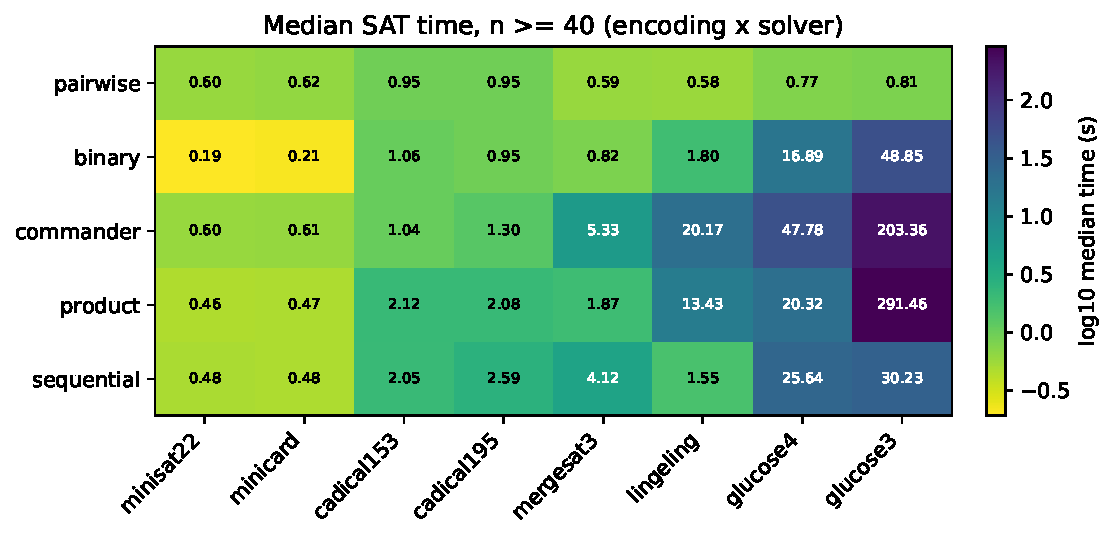
\includegraphics[width=\linewidth]{heatmap_encoding_solver}
  \caption{Median SAT solving time ($n\geq 40$) for each encoding--solver pair;
  darker is slower. Missing cells correspond to configurations in which all runs
  timed out.}
  \label{fig:heatmap}
\end{figure}

Figure~\ref{fig:by_encoding} shows the time as a function of $n$ for each
encoding with one curve per solver. The curves for pairwise are tightly
clustered, indicating robustness across solvers, whereas the other encodings
diverge strongly as $n$ grows, with the Glucose curves rising several orders of
magnitude above the rest.

\begin{figure*}[t]
  \centering
  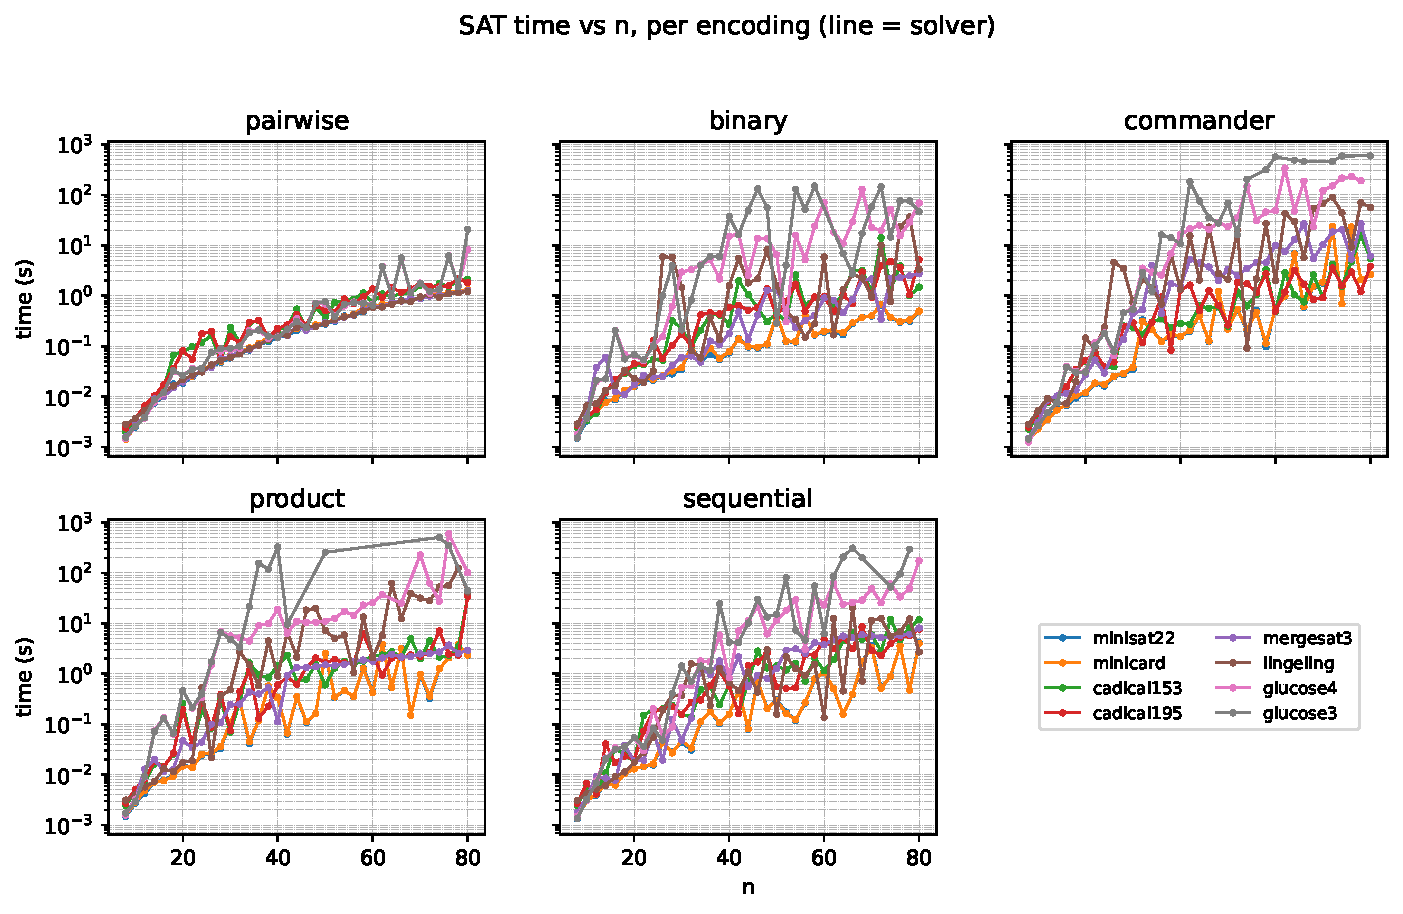
\includegraphics[width=\textwidth]{solver_by_encoding}
  \caption{SAT solving time versus $n$ for each encoding (line = solver). The
  pairwise panel is the most uniform; the remaining panels separate strong and
  weak solvers.}
  \label{fig:by_encoding}
\end{figure*}

\subsection{Comparison with MIP and CP}
Table~\ref{tab:baseline} and Figure~\ref{fig:baselines} report the MIP/CP
baselines. Gurobi is by far the fastest, with an almost constant runtime of about
$0.005$\,s regardless of $n$; CPLEX MIP is second at roughly $0.1$\,s for
$n=80$. CP-SAT and CPLEX CP grow more noticeably, while the SCIP- and CBC-based
MIP baselines are slower and noisier.

\begin{table}[t]
\centering
\caption{Median solving time (s) of the MIP/CP baselines.}
\label{tab:baseline}
\begin{tabular}{lrrrrrrr}
\toprule
n & gurobi & cplex\_mp & cpsat & cplex\_cp & mip\_scip & mip\_cbc & pulp\_cbc \\
\midrule
16 & 0.004 & 0.011 & 0.029 & 0.058 & 0.089 & 2.287 & 3.438 \\
24 & 0.003 & 0.012 & 0.037 & 0.089 & 0.087 & 0.081 & 0.168 \\
32 & 0.004 & 0.021 & 0.076 & 0.103 & 0.133 & 0.131 & 0.320 \\
40 & 0.004 & 0.029 & 0.108 & 0.134 & 2.603 & 0.367 & 0.368 \\
48 & 0.004 & 0.033 & 0.157 & 0.217 & 0.558 & 0.852 & 0.604 \\
56 & 0.005 & 0.041 & 0.201 & 0.264 & 8.414 & 1.086 & 1.265 \\
64 & 0.006 & 0.058 & 0.262 & 0.337 & 15.124 & 1.545 & 1.109 \\
72 & 0.006 & 0.058 & 0.351 & 0.424 & 8.391 & 1.645 & 1.787 \\
80 & 0.005 & 0.098 & 0.474 & 0.609 & 3.170 & 1.284 & 2.749 \\
\bottomrule
\end{tabular}
\end{table}


\begin{figure}[t]
  \centering
  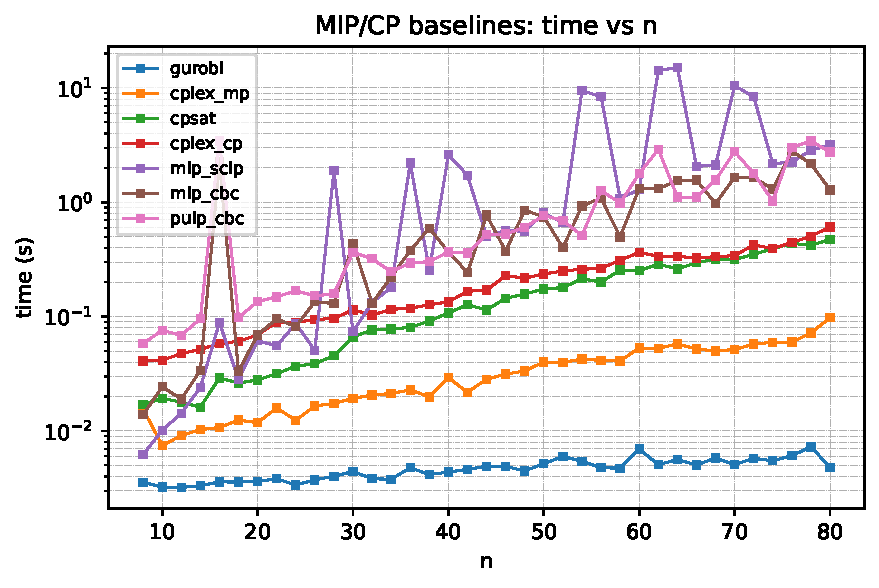
\includegraphics[width=\linewidth]{baselines_time_vs_n}
  \caption{Median solving time of the MIP/CP baselines as a function of $n$.}
  \label{fig:baselines}
\end{figure}

Figure~\ref{fig:comparison} compares the best SAT configuration
(binary encoding with MiniSat) against all baselines. For $n\geq 60$ the best SAT
approach is on the order of $0.3$--$0.9$\,s, comparable to CP-SAT and CPLEX CP
and clearly faster than the CBC/SCIP baselines, but slower than CPLEX MIP and far
slower than Gurobi. The gap to Gurobi widens with $n$.

\begin{figure}[t]
  \centering
  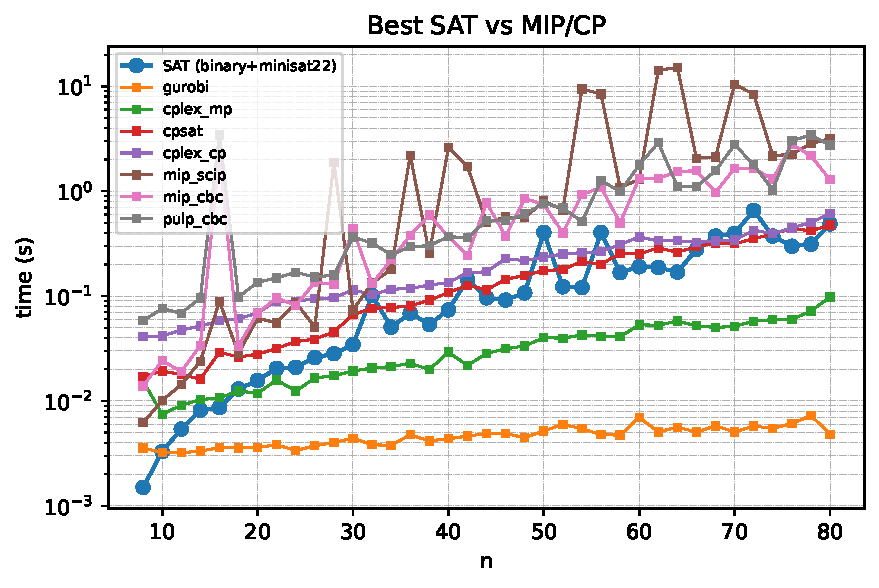
\includegraphics[width=\linewidth]{method_comparison}
  \caption{Best SAT configuration (binary encoding with MiniSat) versus the
  MIP/CP baselines.}
  \label{fig:comparison}
\end{figure}

\subsection{Discussion}
Three observations stand out.
First, the encoding--solver interaction means that encoding quality cannot be
judged in isolation: pairwise wins for propagation-weak solvers because its many
clauses give strong propagation, while binary wins for strong CDCL solvers
because it keeps the formula small. This is consistent with the classical view
that the best encoding depends on the solver \citep{Prestwich2009}.
Second, we observed a solver-specific artefact: for the small pairwise instance
$n=8$, CaDiCaL reports zero decisions, propagations, and conflicts because it
solves the instance entirely during preprocessing, without entering its search
loop; the counters therefore measure search effort only, not total work. This
confirms that propagation-based statistics should be used with care when
comparing heterogeneous solvers.
Finally, the commercial MIP solver Gurobi dominates all other exact approaches on
this feasibility-oriented problem, which highlights that, for tiny feasibility
instances, a tuned MIP presolve and heuristic can outperform a generic SAT
workflow even when the latter is carefully encoded. The advantage of SAT is its
modularity: the same model runs with many solvers and encodings, and the best
configuration remains competitive with CP-SAT and CPLEX CP.

\section{Conclusion}\label{sec:conclusion}
We presented an exact SAT-based approach for N-Queens, implemented with five
hand-written and seven PySAT cardinality encodings and eight SAT solvers, and
compared it with seven MIP/CP baselines. Our experiments show a strong
encoding--solver interaction, identify MiniSat and MiniCard as the most effective
solvers and pairwise and binary as the best encodings depending on the solver,
and confirm the strength of commercial MIP on this problem. Future work includes
extending the study to the optimisation variant of N-Queens (maximising the
number of queens on an $n\times m$ board), to harder unsatisfiable instances, and
to additional SAT solvers once the crashing and missing solvers become available.

\section*{Declaration of generative AI and AI-assisted technologies in the
manuscript preparation process}
During the preparation of this work the author used a large language model to
assist with code development, text drafting, and language revision. After using
this tool, the author reviewed and edited the content as needed and takes full
responsibility for the content of the publication.

\bibliographystyle{cas-model2-names}
\bibliography{../refs}

\section*{Research Data}
The source code, benchmark data, and the scripts that reproduce all figures and
tables are available at:
\begin{center}
\url{https://github.com/Duc-2705/n-Queens}
\end{center}

\end{document}
